%% ----------------------------------------------------------------
%% Thesis.tex -- MAIN FILE (the one that you compile with LaTeX)
%% ---------------------------------------------------------------- 

% Set up the document
\documentclass[a4paper, 11pt, oneside]{Thesis}  % Use the "Thesis" style, based on the ECS Thesis style by Steve Gunn
% \graphicspath{./Images/}  % Location of the graphics files (set up for graphics to be in PDF format)

% Include any extra LaTeX packages required
\usepackage[square, numbers, comma, sort&compress]{natbib}  % Use the "Natbib" style for the references in the Bibliography
\usepackage{verbatim}  % Needed for the "comment" environment to make LaTeX comments
\usepackage{vector}  % Allows "\bvec{}" and "\buvec{}" for "blackboard" style bold vectors in maths
\hypersetup{urlcolor=blue, colorlinks=true}  % Colours hyperlinks in blue, but this can be distracting if there are many links.

%% ----------------------------------------------------------------
\begin{document}
\frontmatter      % Begin Roman style (i, ii, iii, iv...) page numbering

% Set up the Title Page
\title  {Skylab: NUS Orbital Project Platform}
\authors  {\texorpdfstring
	{\href{mailto:franklingujunchao@gmail.com}{Gu Junchao}}
	{Gu Junchao}}
\addresses  {\groupname\\\deptname\\\univname}  % Do not change this here, instead these must be set in the "Thesis.cls" file, please look through it instead
\date       {\today}

\maketitle
%% ----------------------------------------------------------------

\setstretch{1.3}  % It is better to have smaller font and larger line spacing than the other way round

% Define the page headers using the FancyHdr package and set up for one-sided printing
\fancyhead{}  % Clears all page headers and footers
\rhead{\thepage}  % Sets the right side header to show the page number
\lhead{}  % Clears the left side page header

\pagestyle{fancy}  % Finally, use the "fancy" page style to implement the FancyHdr headers

\makedoctitle

%% ----------------------------------------------------------------
% Declaration Page required for the Thesis, your institution may give you a different text to place here
\setcounter{page}{1}
\Declaration{

\addtocontents{toc}{\vspace{1em}}  % Add a gap in the Contents, for aesthetics

I, Gu Junchao, declare that this thesis titled, `Skylab: NUS Orbital Project Platform' and the work presented in it are my own. I confirm that:

\begin{itemize} 
\item[\tiny{$\blacksquare$}] This work was done wholly or mainly while in candidature for a bachelor's degree at this University.
 
\item[\tiny{$\blacksquare$}] Where any part of this thesis has previously been submitted for a degree or any other qualification at this University or any other institution, this has been clearly stated.
 
\item[\tiny{$\blacksquare$}] Where I have consulted the published work of others, this is always clearly attributed.
 
\item[\tiny{$\blacksquare$}] Where I have quoted from the work of others, the source is always given. With the exception of such quotations, this thesis is entirely my own work.
 
\item[\tiny{$\blacksquare$}] I have acknowledged all main sources of help.
 
\item[\tiny{$\blacksquare$}] Where the thesis is based on work done by myself jointly with others, I have made clear exactly what was done by others and what I have contributed myself.
\\
\end{itemize}
 
 
Signed:\\
\rule[1em]{25em}{0.5pt}  % This prints a line for the signature
 
Date:\\
\rule[1em]{25em}{0.5pt}  % This prints a line to write the date
}
\clearpage  % Declaration ended, now start a new page

%% ----------------------------------------------------------------
% The "Funny Quote Page"
\pagestyle{empty}  % No headers or footers for the following pages

\null\vfill
% Now comes the "Funny Quote", written in italics
\textit{``If debugging is the process of removing software bugs, then programming must be the process of putting them in.''}

\begin{flushright}
Edsger Dijkstra
\end{flushright}

\vfill\vfill\vfill\vfill\vfill\vfill\null
\clearpage  % Funny Quote page ended, start a new page
%% ----------------------------------------------------------------

% The Abstract Page
\addtotoc{Abstract}  % Add the "Abstract" page entry to the Contents
\abstract{
\addtocontents{toc}{\vspace{1em}}  % Add a gap in the Contents, for aesthetics

Orbital is the School of Computing`s self-driven programming summer experience. It is designed to give first-year students the opportunity to self-learn and build something useful\cite{citation0}. As more and more students join Orbital program, administration of the program and evaluations among teams are becoming increasingly complex and challenging. Therefore, Skylab is designed and implemented to help students to submit project logs and evaluate other teams with ease as well as to help the administrator of Orbital program overlook and manage this module well. In this project, we find and solve real-life problems faced by students, advisors, facilitators and administrators of Orbital program with an extensible system design and continuous contribution in an agile software development process.

\begin{flushleft}
{\normalsize \textbf{Subject descriptors:} \par}
{\normalsize \subjectname \par}
{\normalsize \textbf{Keywords:} \par}
{\normalsize \keywordnames \par}
\end{flushleft}
}

\clearpage  % Abstract ended, start a new page
%% ----------------------------------------------------------------

\setstretch{1.3}  % Reset the line-spacing to 1.3 for body text (if it has changed)

% The Acknowledgements page, for thanking everyone
\acknowledgements{
\addtocontents{toc}{\vspace{1em}}  % Add a gap in the Contents, for aesthetics

I would like to express my most sincere appreciation to my project supervisor and project
administrator, Assoc Prof Min-Yen Kan. Throughout this project, it was him who tirelessly
provided me with significant support and assistance. I would also like to appreciate facilitators, advisers and students in Orbital program for suggesting many useful features and bringing up issues to make Skylab more usable.

}
\clearpage  % End of the Acknowledgements
%% ----------------------------------------------------------------

\pagestyle{fancy}  %The page style headers have been "empty" all this time, now use the "fancy" headers as defined before to bring them back


%% ----------------------------------------------------------------
\lhead{\emph{Contents}}  % Set the left side page header to "Contents"
\tableofcontents  % Write out the Table of Contents

%% 
% End of the pre-able, contents and lists of things
% Begin the Dedication page

\setstretch{1.3}  % Return the line spacing back to 1.3

\addtocontents{toc}{\vspace{2em}}  % Add a gap in the Contents, for aesthetics


%% ----------------------------------------------------------------
\mainmatter	  % Begin normal, numeric (1,2,3...) page numbering
\pagestyle{fancy}  % Return the page headers back to the "fancy" style

% Include the chapters of the thesis, as separate files
% Just uncomment the lines as you write the chapters

\chapter{Introduction}

Orbital is the School of Computing’s self-driven programming summer experience. It is designed to give first-year students the opportunity to self-learn and build something useful. It is designed as a 4 modular credit (MC) module that is taken pass/fail (CS/CU) over the summer. With its focus on hands-on experience, it has been catching more and more attention and an increasing number of year-one students are joining the program to code something useful and interesting. During the academic year of 2015-2016, more than 250 students completed Orbital program.

For the evaluation of Orbital program, students are supposed to submit to Milestones as a team, stating what they have done during that phase. And then assigned peer teams(each team will be assigned for about 3 peer teams) will be giving feedback regarding the submission and the application built by the team of students. At the same time, there will be an adviser who will overlook the whole process and provide evaluation of a team's submission too. After 3 submissions and evaluations are done, a feedback is expected from a team to its peer teams and its adviser regarding the quality of evaluations received.

The nature of Orbital defines the scope of Skylab —- A development project built for peer evaluations. It also provides students with a real-life Software Engineering training ground to learn and sharpen programming and system design skills. 

\section{Challenges}

\subsection{System design}
Skylab is built on top of Ruby on Rails, a mature convention-over-configuration web framework. So the first challenge for me is to get familiar with the conventions and recommended ways of doing things in Rails community. Then I can design the web application on the top of main-stream philosophy in Rails community. Another issue with the design of Skylab is that this is the first time I have been designing such an application from ground up, without any guidance from any experienced Ruby on Rails developers. Therefore, it is all about try-and-error and explore my own way. Reading books and browsing on-line tutorials helped me a lot and luckily there are plenty of resources about Ruby on Rails development due to its popularity.

\subsection{Evolving requirements}
Although the scope of the project is very clear and well-defined, changes in requirements are expected and did happen a lot due to evolving features of Skylab project and Skylab users' feedback. The challenge is to cope with all changes and sometimes adjustments to the design of system have to be made to accommodate for extensions. Therefore agility in development and adaptability of the system is expected.

\subsection{Data migration}
Sometimes schema migration is required as a result of change in requirements. Therefore, dealing with old data and migration of data without affecting the use of application is another challenge during the development of Skylab. Extreme attention when migrating is required as data may not be clean enough and careless migration may even cause the system to be unusable for some users.

\subsection{Security}
Security is definitely a very important perspective in web development. Although Rails is handling security well by taking measures against SQL injection, XSS attacks and CSRF attacks, there are still quite some vulnerabilities if not handled well. During development of Skylab, various techniques and practices are adopted to make Skylab more secure and trust-able. What is more, with different roles in Skylab, a role based access control system is in place for permitting users to carry out allowed actions only.

\subsection{Coding quality/maintainability}
Although currently there is only me constantly contributing to Skylab repository, a good development cycle which is agile enough is not only important for me to keep track of history and manage different issues but also convenient for developers who will join later to jump in and get started. Testing is also a very important factor when it is comes to long-term maintenance. A continuous integration would also help me in catching regression errors in development early and easily. Besides all mentioned above, refactoring is helping in the growth of the project.

\section{Objectives}

In this project, I need to:
\begin{itemize}
  \item Enable users to login via NUS OpenID if they have NUS Net IDs already.
  \item Enable users to login via combination of email and password for those who do not have NUS Net IDs and also serve as a backup solution to NUS OpenID login.
  \item Enable students to edit their own team's details including ``Team Name'' and ``Project Level''.
  \item Enable students to submit for Milestones or edit their previous submissions. Besides, students in the same team should be able to see changes made by teammates.
  \item Enable students to view submissions from teams that they should evaluate(For example, Team A is supposed to evaluate Team B and Team C; Then students in Team A should be able to view submissions from Team B and Team C).
  \item Enable students to submit peer evaluations for submissions from teams that they are evaluating.
  \item Enable students to view peer evaluations from teams that are evaluating their own teams and their adviser(For example, Team B is supposed to be evaluated by Team A and Team C; Then students in Team B should be able to view peer evaluations submitted by Team A and Team C for Team B). For public part of a peer evaluation, students can see response with name of the team that submitted that evaluation; As for private part, students can only see a compilation of all private part responses without team names.
  \item Enable students to submit feedback to evaluate the evaluations received(For example, Team B is supposed to be evaluated by Team A and Team C; Then students in Team B should be able to submit feedback to Team A and Team C regarding peer evaluations received from each team).
  \item Enable advisers to view a list of all teams under his/her supervision and edit any of these team's details including ``Team name'', ``Project Level'' and ``Has Dropped''.
\end{itemize}

\section{Outline}

In this report, I will discuss various accomplishments I have done in the development. Chapter 2 will be an overview of current architecture of Skylab, and methodologies I employed during the development. Chapter 3, 4 and 5 will be talking about problems in the implementation of submissions, peer evaluations and feedback. Then security related issues such as user authentication and access control will be discussed in Chapter 6. Chapter 7 is about adviser focus group meeting and its findings. Last but not least, a summary of work and an overlook of future development will come in Chapter 8.
 % Introduction

\chapter{Background} \label{background}

Skylab is built using Ruby on Rails, a well-known web development framework with a great support from a large community, used widely in the industries by companies like Twitter, Groupon, Bloomberg, Airbnb and many more\cite{citation1}. There are many reasons why we have chosen Ruby on Rails. Firstly, Ruby is clean, elegant and easy to read and this feature enables programmers to be more productive. Secondly, Ruby on Rails is adopting many advanced industrial conventions and this enables contributors to have good exposure to programming in the industry. What is more, scaffolding and many gems can significantly boost the productivity. Last but not least, Ruby on Rails community has a favor for open source contribution which aligns well with the open source nature of Skylab.

For the selection of database, we used PostgreSQL. Part of the reason is that it is open source and quite mature, with good drivers available in many languages\cite{citation2}. Besides, we need full ACID compliance for consistency of data and we do not need scalability to multiple servers in the foreseeable future. And PostgreSQL has recently added implementation for rich data structures such as JSON which would make development much easier\cite{citation3}.

Puma is the web server we have chosen for Skylab. Among Passenger, Unicorn, Rainbows! and Puma, Puma is considered to be fast and memory friendly according to online benchmarking\cite{citation4}. Puma is built for high-concurrency and speed and more and more developers to switching to Puma in Rails community\cite{citation5}.

We have selected Nginx as our HTTP server. Nginx has grown in popularity since its release due to its light-weight resource utilization and its ability to scale easily with low memory usage. It excels at serving static content quickly and is designed to pass dynamic requests off to other software that is better suited for those purposes\cite{citation6}. There are also some benchmarking results that indicate the superiority in Nginx handling concurrent access and low memory usage of Nginx\cite{citation7}.

A high-level overview of the architecture of Skylab is illustrated in Figure~\ref{fig:Skylabarch}. Incoming requests to server will first be forwarded to Puma worker processes by Nginx. After that the corresponding Skylab code in Ruby on Rails framework will be executed and when accessing database is required, PostgreSQL will come into picture and serve the data. 

\begin{figure}[h]
  \centering
  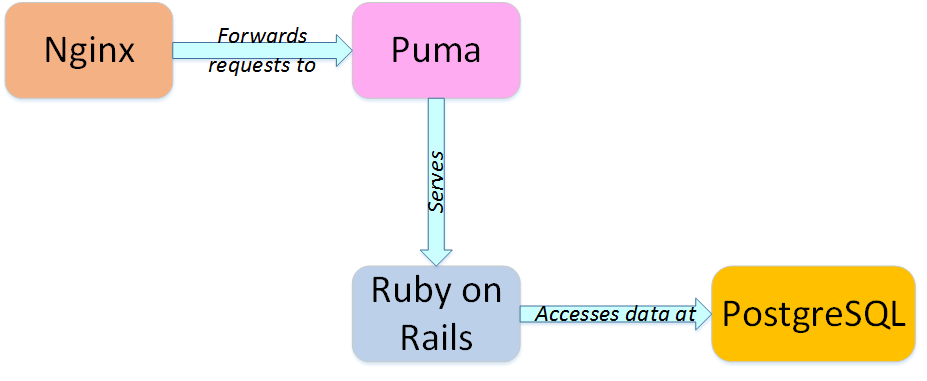
\includegraphics[width=0.85\textwidth]{Images/Skylab_arch.png}
  \caption{Architecture of Skylab}
  \label{fig:Skylabarch}
\end{figure}

\section{System design}

The basic MVC structure of Rails is shown in Figure~\ref{fig:RailsMVC}\cite{citationMVC}:

\begin{figure}[h]
  \centering
  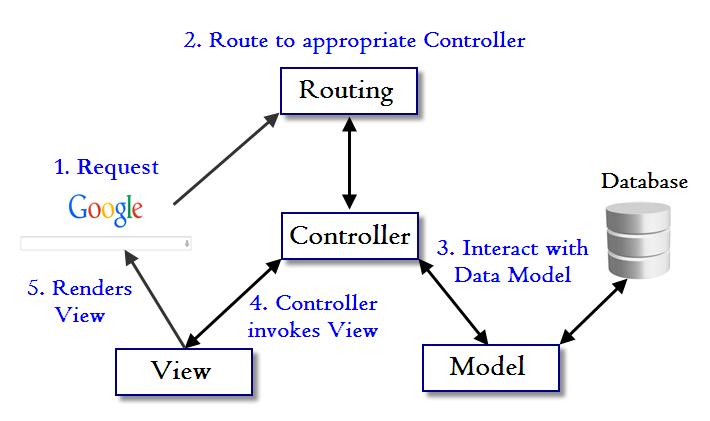
\includegraphics[width=0.85\textwidth]{Images/Rails_MVC.png}
  \caption{Illustration of how MCV works in Rails}
  \label{fig:RailsMVC}
\end{figure}

After request is received by Ruby on Rails framework, the router will look at the pattern of the requested URL path and send it to the corresponding method of the target controller class. The controller is supposed to query models and gather necessary information for rendering the view for user. Last but not least, the response will be sent back to user for viewing.

So the most fundamental component in this whole process is model, which stores all the business data. A good design of model can in fact save a lot of trouble when it comes to writing controller code.

\begin{figure}[h]
  \centering
  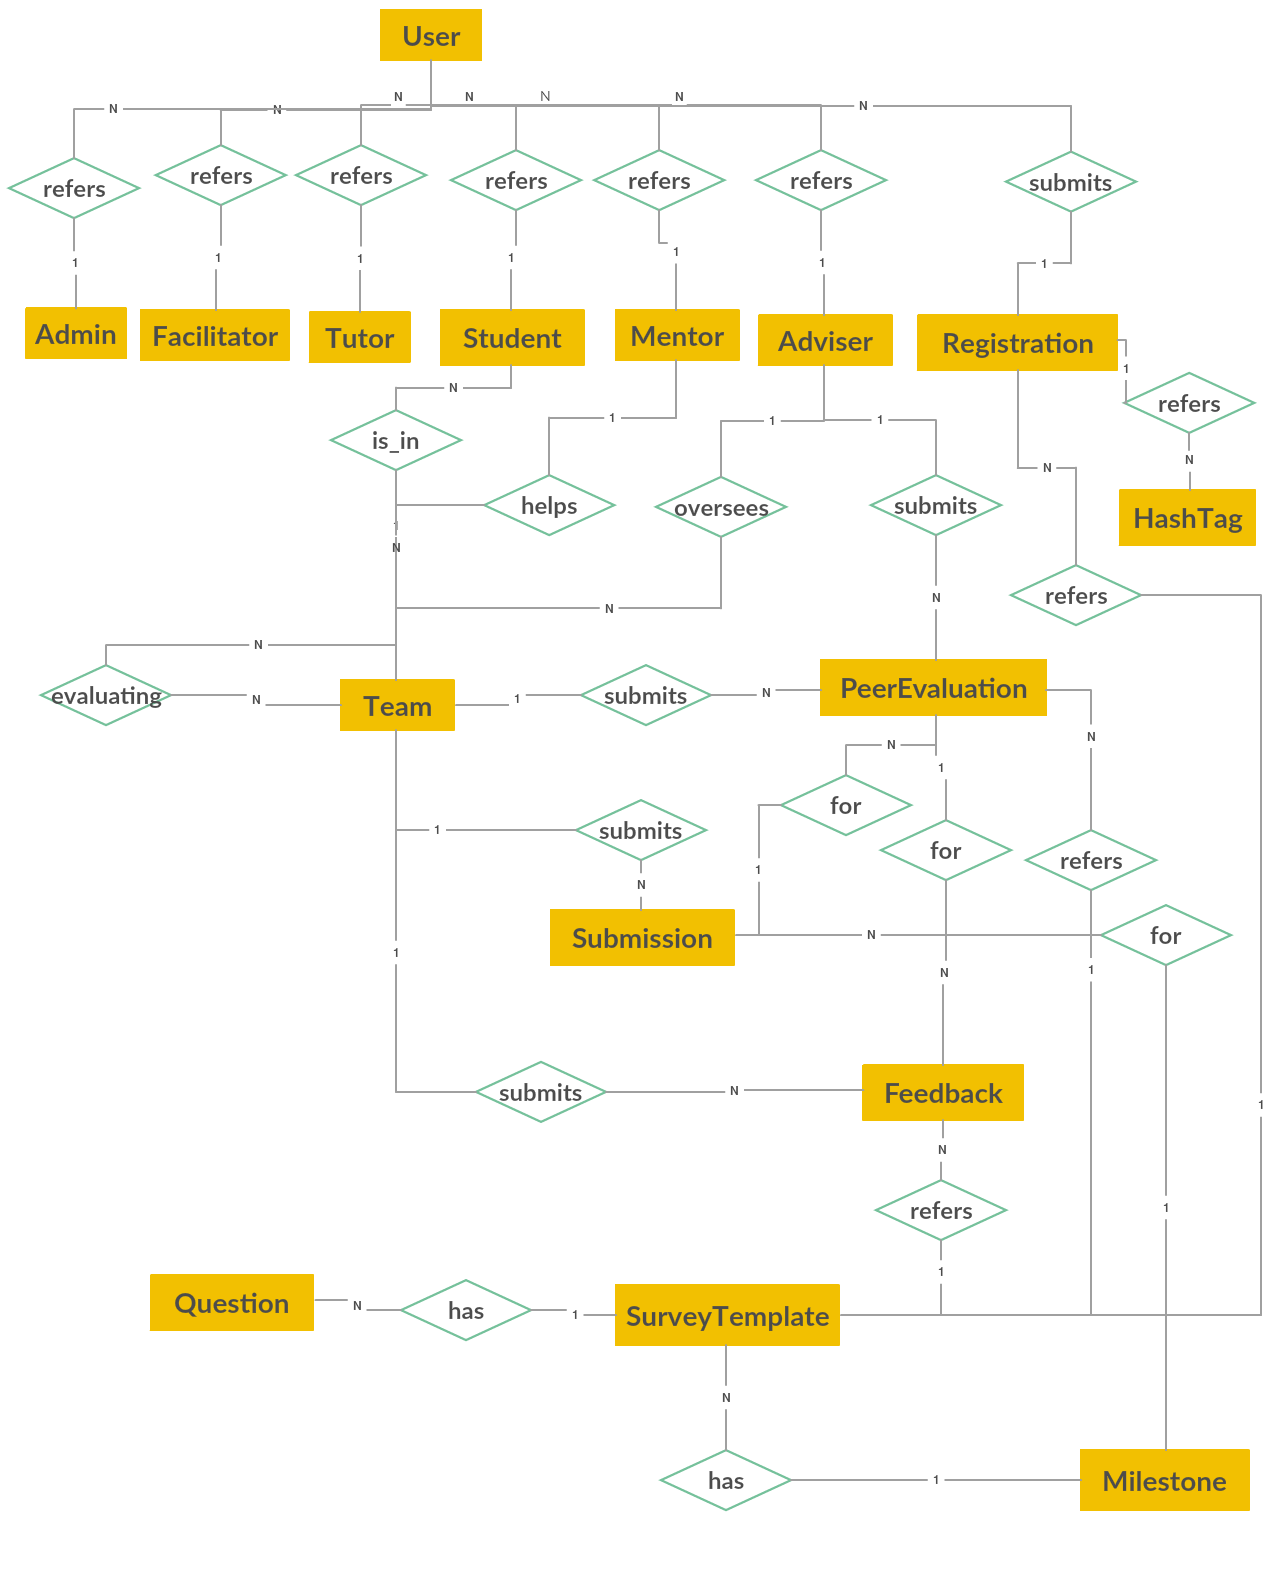
\includegraphics[width=\textwidth]{Images/Skylab_ER.png}
  \caption{Current ER diagram for Skylab}
  \label{fig:SkylabER}
\end{figure}

As you can see from the entity relation diagram shown in Figure~\ref{fig:SkylabER}, users' basic information is captured in the \textit{User} model and each user may have different roles such as \textit{Admin}, \textit{Student}, \textit{Adviser}, \textit{Mentor}. Each student has a \textit{Team} and a team has an \textit{Adviser} and a \textit{Mentor}. Each team will create \textit{Submissions} to \textit{Milestones} to report their progress and assigned evaluator teams will submit \textit{PeerEvaluations} to their \textit{Submissions}. A \textit{SurveyTemplate} contains \textit{Questions} for a \textit{Feedback}, which is for evaluated team to provide feedback to their evaluator teams.

Controllers are crucial in powering a Rails application and in Skylab we have well-defined controllers to carry different tasks. A list of controllers is as follows:

\begin{itemize}
  \item \textbf{AdminsConroller}: handles listing of all Admins, display of an Admin, creation and update of an Admin as well as deletion of an Admin.
  \item \textbf{AdvisersConroller}: handles listing of all Advisers, display of an Adviser, creation and update of an Adviser as well as deletion of an Adviser.
  \item \textbf{EvaluatingsConroller}: handles listing of all evaluation relationships, creation and update of an evaluation relationship as well as deletion of evaluation relationship.
  \item \textbf{FeedbacksConroller}: handles creation and update of a Feedback.
  \item \textbf{HomeConroller}: handles serving of homepage.
  \item \textbf{MentorsConroller}: handles listing of all Mentors, display of a Mentor, creation and update of a Mentor as well as deletion of a Mentor.
  \item \textbf{MilestonesConroller}: handles listing of all Milestones, display of a Milestone, creation and update of a Milestone as well as deletion of a Milestone.
  \item \textbf{PeerEvaluationsConroller}: handles creation and update of a PeerEvaluation.
  \item \textbf{ReceivedEvalsConroller}: handles listing of all received peer evaluations by a team for one milestone.
  \item \textbf{ReceivedFeedbacksConroller}: handles listing of all received feedbacks by a team for one milestone.
  \item \textbf{StudentsConroller}: handles listing of all Students, display of a Student, creation and update of a Student as well as deletion of a Student.
  \item \textbf{SubmissionsConroller}: handles display of a Submission, creation and update of a Submission.
  \item \textbf{SurveyTemplatesConroller}: handles listing of all SurveyTemplates, creation and update of a SurveyTemplate as well as deletion of a SurveyTemplate.
  \item \textbf{TeamsConroller}: handles listing of all Teams, display of a Team, creation and update of a Team as well as deletion of a Team.
  \item \textbf{UsersConroller}: handles listing of all Users, display of a User, creation and update of a User as well as deletion of a User.
  \item \textbf{auth}: handles authentication related to Devise and OpenID.
  \item \textbf{public\_views}: handles serving of publicly available information.
\end{itemize}

\section{Development process}

As Skylab is a web application for which version does not mean anything in particular, we have adopted GitHub flow in our development process\cite{citation8}. So the master branch always contains the latest stable and deployable code base. Each feature will be developed on a feature branch and once the feature is ready, a pull request is created against master. After code review and all tests passes, pull requests will be merged into master and ready for deployment. Figure~\ref{fig:GithubFlow} illustrates the process as well\cite{citation8}.

\begin{figure}[h]
  \centering
  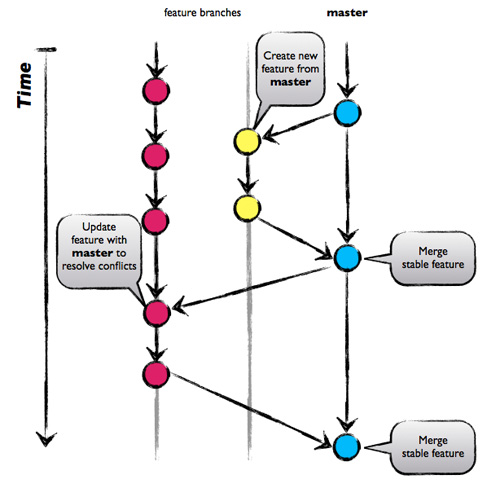
\includegraphics[width=0.7\textwidth]{Images/Github_Flow_Branching_Model.jpg}
  \caption{Branching diagram for GitHub Flow}
  \label{fig:GithubFlow}
\end{figure}

By using GitHub flow and services such as Travis as the continuous integration service, CodeClimate as the code quality monitoring service, we can keep the development of Skylab agile and fast. Besides GitHub flow has enabled Skylab to deployed regularly, which is essential for timely improvement of user experience\cite{citation9}.
 % Background

\chapter{Submission}

Students in Orbital are supposed to report their progress regarding their project for each milestone and they will be therefore submit submissions to describe what they have done. Basically a submission contains 3 parts:

\begin{itemize}
  \item Read me: highlights what are the changes and new features in the project.
  \item Project Log: a summary of work done during the phase and time used for each task.
  \item Video link: a link to a video introducing the project to evaluators.
\end{itemize}

As the structure of \textit{Read me} and \textit{Project Log} is free and we should allow creativity of students when it comes to describing their own projects, we decided to support rich text for submissions and there are some issues coming along this decision. What is more, during use of Skylab, many good suggestions were brought up students and advisers and this brings user experience issue.

\section{Handling of rich text}
We used TinyMCE to support rich text editing feature in Skylab as it is a very popular WYSIWYG editor with a rich set of features\cite{citation10}. There are some libraries with markdown syntax supported such as EpicEditor, Vue.js and Hallo.js which are more lightweight. However, as Skylab is built for freshmen to get more hands-on experience with coding and we do not expect students to be equipped with much prior knowledge such as markdown syntax, markup based editors such as TinyMCE and CKEditor do not require any learning and are easily to get started with. What is more, the large community using TinyMCE has made various plug-ins available for different features. There are also quite resources online about integrating TinyMCE editor in a Rails project. Therefore, we decided to use TinyMCE for \textit{Submissions}' rich text support.

One particular disadvantage of using TinyMCE is that the size of this editor is pretty large and loading of the page will be slowed down because of it. Therefore, TinyMCE related resources is only loaded if the page is requiring rich text editing. This is done by configuration to disable auto loading of all JavaScript, which is the default behavior of Rails. In this way, most pages can stilled by loaded in a very short time.

Rails has built checking against SQL injection attacks and therefore Skylab is safe from such attacks when storing submissions' contents\cite{citation11}. However, there is still currently a known bug in the implementation when it comes to viewing of submissions. As contents like \textit{Read me} and \textit{Project Log} should be rendered as rich text, it is possible for students to carry out XSS attacks by injecting executable JavaScript code in the submission. This sort of vulnerabilities will be fixed in the future.

\section{Usability}
% target milestone selection: manual to js selection to auto selection; adjustment of field orders, auto expansion, auto linking of videos, back to top button

Skylab is a software engineering project and therefore improvement in user experience is one key part when it comes to implementation. During the use of Skylab, many suggestions were brought up by students and advisers about usability. And by addressing these issues, Skylab is serving users better with a smoother user experience.

\subsection{Target Milestone Selection}

When Skylab was used for the first time, students were expected to choose the target milestone, which the submission is for. However, many students reported that it is just a redundant step as every time they will only submit to the currently active milestone. After hearing this, a quick fix of automatically selecting the current milestone for students using JavaScript functions was done, while the manual selection is still possible. And then during the \textit{Adviser Focus Group Meeting}, some advisers further pointed out that the selection should not even be presented to users as it is of completely no use and therefore the whole selection was completely removed from Skylab after the meeting by moving the task to the backend logic. 

\subsection{Rich Text Editing}

As quite some students want to insert image to \textit{Read me} sections, an image uploading feature was soon added to submission page for users' convenience. Behind the scene Skylab is using a third-party API from Imgur. This was done mainly for 2 reasons: Using Imgur is relatively easy to implement; We can also avoid heavy server load due to file uploading and possible attacks in uploaded files.

Another improvement over user experience is auto expanding of TinyMCE editing area as feedback from students mentioned that their \textit{Read me} and \textit{Project Log} are usually quite lengthy. So auto expanding would not require too much scrolling during creating/editing a submission.
 % Orbital workflow

\chapter{Peer Evaluation}
 
\section{Loading of different evaluation templates}

\section{Storing the response}

\section{Usability}
 % Public profile

\chapter{Feedback}
 
\section{Survey template system}

\section{Question creation and storing of response}
 % Security

\chapter{Feedback}
 
\section{Survey template system}

\section{Question creation and storing of response}
 % Testing

\chapter{Adviser focus group meeting}

A focus group is a form of qualitative research in which a group of people are asked about their perceptions, opinions, beliefs, and attitudes towards a product, service, concept, advertisement, idea, or packaging\cite{citation15}. During mid of the semester a focus group meeting about Skylab with 2 advisers was conducted to get advisers' suggestions and feedback on experience with Skylab. The feedback is generally positive while there are indeed some useful suggestions and findings.

\section{Focus group meeting}

The focus group was conducted on 7th Oct 2015 and 3 questionnaires were designed beforehand to get advisers' opinions. During the meeting, discussions about the complete use case flow of Skylab were done and the whole meeting was recorded as well for later reference. Suggestions mentioned in the discussion and described in the responses to questionnaires are listed below, which are also documented in Skylab's repository:

\begin{itemize}
  \item Checking who had already evaluated / or sent feedback on an evaluation: we should have status columns(similar to ``dropped'' status) for submission status, peer evaluation status so that with just one glance adviser can figure out who have not submitted and remind them
  \item Change tab order for adviser homepage: move the current first tab to last as advisers rarely use them
  \item Forms too verbose Three radio fields take up more than one page. Suggested way of presenting options: Poor 1[?] 2[?] 3[?] 4[?] 5[?] Best(Question mark means only after the user hovers over the detailed explanation for the option will be given)
  \item Hosting of videos
  \item Auto expand text boxes when close to full
  \item Dropdown for team selection not clear about whether the new team is being evaluation
  \item Autosave text and input / prompt for leaving page
  \item Summary composite page for the EG with respect to each evaluation question for Likert scale and textboxes / Quick Fix: use anchors to jump to a particular form on a concatenated page.
  \item ``More info'' tab in adviser homepage is misleading
  \item Enable users to view all past submissions, all past peer evaluations(by providing link to viewing them in some place) when you are editing/submitting a peer evaluation.
  \item Evaluating relationship: explore use of D3(or similar stuff) to represent all relationships as graph
\end{itemize}

Besides these suggestions, some of our assumptions have been tested as well and therefore necessary adjustments to plan for future implementation were made according to some of the findings from the focus group meeting.
 % Focus group meeting

\chapter{Conclusion and future work} \label{conclusionandfuturework}

\section{Conclusion}

Most core functionalities have been implemented for Skylab including Submissions, Peer Evaluations, Feedback. However, as pointed in previous discussions as well, issues in security, usability and system design do exist as well and those issues will be addressed in the the coming semester. Besides, more features are expected of Skylab as well to make it serve Orbital program better such as registration of interest, mailer as reminders for deadlines and logging of user activities.

\section{Future work}

A proposed set of major features to be completed in the future for Skylab:

\begin{itemize}
  \item Questions/template system(involving migration of current data): currently \textit{Feedback} is utilizing the \textit{SurveyTemplate} and \textit{Question} system but \textit{Peer Evaluation} and \textit{Submission} are still not. With migration to \textit{Questions} system we can further improve the system by adding more extensibility.
  \item Public view of projects \& teams \& students: listing of previous projects as evidence of work from alumni of Orbital program can also help to attract more freshmen joining.
  \item Registration and post Orbital feedback: As part of Orbital program, registration of interest and post Orbital feedback should be captured in Skylab as well.
  \item Implementation of cohort: Orbital is held every year and certainly Skylab is expected to take cohort into consideration and allow historical records to be captured in the database.
  \item Implementation of more mailer actions: we can explore power of emails by sending reminder emails to students when deadlines are approaching or even embed secure link for students to do submissions without login.
  \item Logging of user activities: by logging down activities carried out by different users, users can more easily figure out what has happened and get a better sense of the context of Skylab.
\end{itemize}

 % Conclusion

%% ----------------------------------------------------------------
% Now begin the Appendices, including them as separate files

\addtocontents{toc}{\vspace{2em}} % Add a gap in the Contents, for aesthetics

\appendix % Cue to tell LaTeX that the following 'chapters' are Appendices

% \chapter{An Appendix}

Lorem ipsum dolor sit amet, consectetur adipiscing elit. Vivamus at pulvinar nisi. Phasellus hendrerit, diam placerat interdum iaculis, mauris justo cursus risus, in viverra purus eros at ligula. Ut metus justo, consequat a tristique posuere, laoreet nec nibh. Etiam et scelerisque mauris. Phasellus vel massa magna. Ut non neque id tortor pharetra bibendum vitae sit amet nisi. Duis nec quam quam, sed euismod justo. Pellentesque eu tellus vitae ante tempus malesuada. Nunc accumsan, quam in congue consequat, lectus lectus dapibus erat, id aliquet urna neque at massa. Nulla facilisi. Morbi ullamcorper eleifend posuere. Donec libero leo, faucibus nec bibendum at, mattis et urna. Proin consectetur, nunc ut imperdiet lobortis, magna neque tincidunt lectus, id iaculis nisi justo id nibh. Pellentesque vel sem in erat vulputate faucibus molestie ut lorem.

Quisque tristique urna in lorem laoreet at laoreet quam congue. Donec dolor turpis, blandit non imperdiet aliquet, blandit et felis. In lorem nisi, pretium sit amet vestibulum sed, tempus et sem. Proin non ante turpis. Nulla imperdiet fringilla convallis. Vivamus vel bibendum nisl. Pellentesque justo lectus, molestie vel luctus sed, lobortis in libero. Nulla facilisi. Aliquam erat volutpat. Suspendisse vitae nunc nunc. Sed aliquet est suscipit sapien rhoncus non adipiscing nibh consequat. Aliquam metus urna, faucibus eu vulputate non, luctus eu justo.

Donec urna leo, vulputate vitae porta eu, vehicula blandit libero. Phasellus eget massa et leo condimentum mollis. Nullam molestie, justo at pellentesque vulputate, sapien velit ornare diam, nec gravida lacus augue non diam. Integer mattis lacus id libero ultrices sit amet mollis neque molestie. Integer ut leo eget mi volutpat congue. Vivamus sodales, turpis id venenatis placerat, tellus purus adipiscing magna, eu aliquam nibh dolor id nibh. Pellentesque habitant morbi tristique senectus et netus et malesuada fames ac turpis egestas. Sed cursus convallis quam nec vehicula. Sed vulputate neque eget odio fringilla ac sodales urna feugiat.

Phasellus nisi quam, volutpat non ullamcorper eget, congue fringilla leo. Cras et erat et nibh placerat commodo id ornare est. Nulla facilisi. Aenean pulvinar scelerisque eros eget interdum. Nunc pulvinar magna ut felis varius in hendrerit dolor accumsan. Nunc pellentesque magna quis magna bibendum non laoreet erat tincidunt. Nulla facilisi.

Duis eget massa sem, gravida interdum ipsum. Nulla nunc nisl, hendrerit sit amet commodo vel, varius id tellus. Lorem ipsum dolor sit amet, consectetur adipiscing elit. Nunc ac dolor est. Suspendisse ultrices tincidunt metus eget accumsan. Nullam facilisis, justo vitae convallis sollicitudin, eros augue malesuada metus, nec sagittis diam nibh ut sapien. Duis blandit lectus vitae lorem aliquam nec euismod nisi volutpat. Vestibulum ornare dictum tortor, at faucibus justo tempor non. Nulla facilisi. Cras non massa nunc, eget euismod purus. Nunc metus ipsum, euismod a consectetur vel, hendrerit nec nunc.	% Appendix Title

%\input{Appendices/AppendixB} % Appendix Title

%\input{Appendices/AppendixC} % Appendix Title

\addtocontents{toc}{\vspace{2em}}  % Add a gap in the Contents, for aesthetics
\backmatter

%% ----------------------------------------------------------------
\label{Bibliography}
\lhead{\emph{Bibliography}}  % Change the left side page header to "Bibliography"
\bibliographystyle{unsrtnat}  % Use the "unsrtnat" BibTeX style for formatting the Bibliography
\bibliography{Bibliography}  % The references (bibliography) information are stored in the file named "Bibliography.bib"

\end{document}  % The End
%% ----------------------------------------------------------------
